%%%%%%%%%%%%%%%%%%%%%%%%%%%%%%%%%%%%%%%%%%%%%%%%%%%%%%%%%%%%%%%%%%%%%%%%%%%

\documentclass[a4paper,oneside,12pt]{article}
\usepackage{mystyle}

\begin{document}

\title{\Large\bf Linear functions}
\author{%%
  Minh Van Nguyen \\
  \url{mvngu@gmx.com}
}
\date{\today}
\maketitle

\begin{packeditem}
\item Application of linear equations: fill a bucket with water.
\end{packeditem}

%%%%%%%%%%%%%%%%%%%%%%%%%%%%%%%%%%%%%%%%%%%%%%%%%%%%%%%%%%%%%%%%%%%%%%%%%%%

\section{General form}
\label{sec:general_form}

A \emph{linear function} is an expression of the form
%%
\begin{equation}
\label{eqn:linear_function_general}
f(x)
=
ax + b.
\end{equation}
%%
The numbers $a$ and $b$ are fixed real numbers, while $x$ is a
variable that can be any real number.  What does the function $f(x)$
look like?

As an example, set $a = b = 1$ so that you have $f(x) = x + 1$.  The
graph of $f(x) = x + 1$ is a straight line that passes through the
point $A = \tuple{-1}{0}$ on the $x$-axis and the point
$B = \tuple{0}{1}$ on the $y$-axis.  How were the coordinates of $A$
and $B$ calculated?  For the point $A$, you set $f(x) = 0$ and solve
the equation $0 = x + 1$ for $x$ to get $x = -1$.  The $x$-coordinate
of $A$ is $-1$ and the $y$-coordinate is $0$.  For the point $B$,
you set $x = 0$ and solve the equation $y = 0 + 1$ for $y$ to obtain
$y = 1$.  Then $B$ has $x$-coordinate $0$ and $y$-coordinate $1$.  You
plot the points $A$ and $B$, then draw a straight line through those
two points to produce the graph in \Figure{fig:plot_x_+_1}.

\begin{figure}[!htbp]
\centering
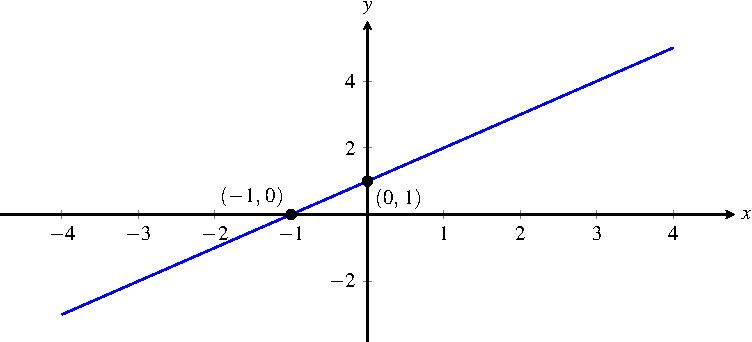
\includegraphics[scale=1]{image/06/a-1-b-1.pdf}
\caption{%%
  A graph of the function $f(x) = x + 1$.
}
\label{fig:plot_x_+_1}
\end{figure}

In general, how would you draw the graph of the
\Function{eqn:linear_function_general}?  As in the example above, you
want to determine two different points of the function $f(x)$.  A
common way to do so is as follows.  You set $f(x) = 0$ and determine
the point $A = \tuple{\alpha}{0}$, where $x = \alpha$ is obtained by
solving $f(x) = 0$ for $x$.  You then set $x = 0$ and determine the
point $B = \tuple{0}{\beta}$, where $\beta = f(0)$.  Plot the points
$A$ and $B$, then draw a straight line through those two points.  The
result is a graph of the \Function{eqn:linear_function_general}.  The
point $A = \tuple{\alpha}{0}$ is called the $x$-intercept because this
is the point where the graph of $f(x) = ax + b$ intersects the
$x$-axis.  Similarly, the point $B = \tuple{0}{\beta}$ is the
$y$-intercept because it is the point where the graph of $f(x)$
intersects the $y$-axis.  Let's put the above strategy into practice.

\begin{example}
Suppose in \Equation{eqn:linear_function_general} you set $a = 2$ and
$b = -1 / 2$.  Draw a graph of the function
$f(x) = 2x - \frac{1}{2}$.
\end{example}

\begin{solution}
To obtain the $x$-intercept $A$, you set $f(x) = 0$ and solve the
equation $0 = 2x - \frac{1}{2}$ for $x$.  The latter equation can be
written as $2x = \frac{1}{2}$ and dividing both sides by $2$ shows
that
%%
\begin{align*}
x
&=
\frac{1}{2} \div 2 \\[4pt]
&=
\frac{1}{2} \times \frac{1}{2} \\[4pt]
&=
\frac{1}{4}.
\end{align*}
%%
The $x$-intercept has coordinates $A = \tuple{\frac{1}{4}}{0}$.  The
coordinates of the $y$-intercept $B$ are determined by first setting
$x = 0$.  You then solve the equation $y = 2 \times 0 - \frac{1}{2}$
for $y$.  The latter equation can be written as
%%
\begin{align*}
y
&=
2 \times 0 - \frac{1}{2} \\[4pt]
&=
0 - \frac{1}{2} \\[4pt]
&=
-\frac{1}{2}
\end{align*}
%%
and you have the $y$-intercept $B = \tuple{0}{-\frac{1}{2}}$.  Plot
the points $A$ and $B$ and draw a straight line through the two points
to produce the graph in \Figure{fig:plot_2x_minus_half}.
\end{solution}

\begin{figure}[!htbp]
\centering
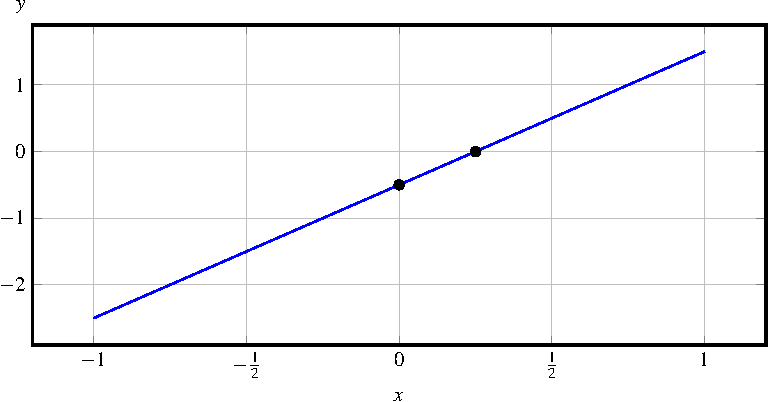
\includegraphics[scale=1]{image/06/a-2-b-minus-half.pdf}
\caption{%%
  A graph of the function $f(x) = 2x - \frac{1}{2}$.
}
\label{fig:plot_2x_minus_half}
\end{figure}

\begin{exercise}
Draw a graph of the function $f(x) = 2x - 2$.
\end{exercise}

\ifbool{showSolution}{
\begin{solution}
You want two different points $A$ and $B$ of the function
$f(x) = 2x - 2$.  A graph of the function is obtained by drawing a
straight line through those two points.  First, you set $f(x) = 0$ and
solve the equation $0 = 2x - 2$ for $x$.  You can write the latter
equation as $2x = 2$ and dividing both sides by $2$ shows that
$x = 1$.  Thus you have the point $A = \tuple{1}{0}$.  Second, you set
$x = 0$ and solve the equation $y = 2 \times 0 - 2$ for $y$.  Write
the last equation as $y = 0 - 2$ and you see that $y = -2$.  Thus you
have the point $B = \tuple{0}{-2}$.  Plot the two points $A$ and $B$,
draw a straight line through those two points, and you have the graph
in \Figure{fig:plot_2x_minus_2}.

\begin{figure}[!htbp]
\centering
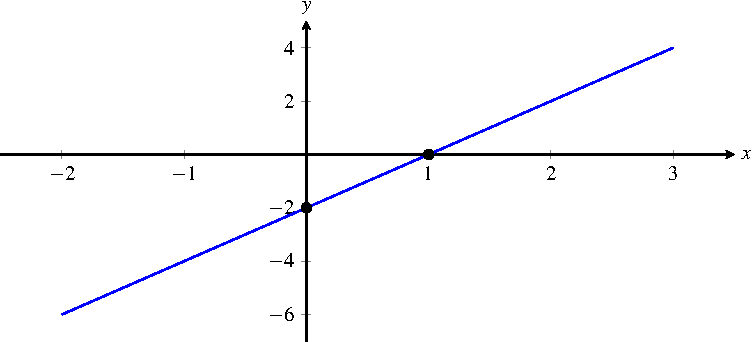
\includegraphics[scale=1]{image/06/a-2-b-minus-2.pdf}
\caption{%%
  A graph of the function $f(x) = 2x - 2$.
}
\label{fig:plot_2x_minus_2}
\end{figure}
\end{solution}
}{}

\begin{exercise}
Draw a graph of the function $f(x) = 3x + \frac{1}{2}$.
\end{exercise}

\ifbool{showSolution}{
\begin{solution}
Determine two points of the function $f(x)$ and draw a straight line
through those two points to produce a graph of the function.  For the
first point, set $f(x) = 0$ and solve the equation
$0 = 3x + \frac{1}{2}$ for $x$.  The latter equation can be written as
$3x = -\frac{1}{2}$.  Multiply both sides by $\frac{1}{3}$ to see that
$x = -\frac{1}{2} \times \frac{1}{3} = -1 / 6$ and you have the point
$A = \tuple{-\frac{1}{6}}{0}$.  For the second point, set $x = 0$ and
solve the equation $y = 3 \times 0 + \frac{1}{2}$ for $y$.  The last
equation can be written as $y = 1 / 2$ and you have the point
$B = \tuple{0}{\frac{1}{2}}$.  Plot the two points and draw a straight
line through those two points to produce the graph in
\Figure{fig:plot_3x_half}.

\begin{figure}[!htbp]
\centering
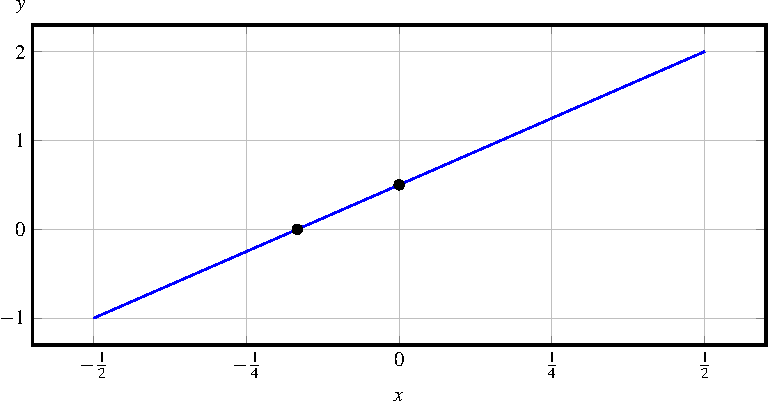
\includegraphics[scale=1]{image/06/a-3-b-half.pdf}
\caption{%%
  A graph of the function $f(x) = 3x + \frac{1}{2}$.
}
\label{fig:plot_3x_half}
\end{figure}
\end{solution}
}{}


%%%%%%%%%%%%%%%%%%%%%%%%%%%%%%%%%%%%%%%%%%%%%%%%%%%%%%%%%%%%%%%%%%%%%%%%%%%

\section{Special cases}

Consider the case where $a = 0$ in
\Equation{eqn:linear_function_general}.  Then you have $f(x) = b$,
which states that no matter what the value of $x$ is you will always
get $y = b$.  For this reason, the function $f(x) = b$ is called a
\emph{constant function}.  The graph of the constant function
$f(x) = b$ is a horizontal line through the point $b$ on the
$y$-axis and this horizontal line is parallel to the $x$-axis.  See
\Figure{fig:constant_functions} for the examples of $b = 2$ and
$b = -3$.

\begin{figure}[!htbp]
\centering
\subfigure[]{
  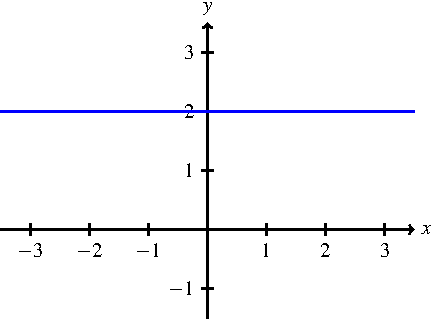
\includegraphics[scale=0.8]{image/06/a-0-b-2.pdf}
}
%%
\qquad
%%
\subfigure[]{
  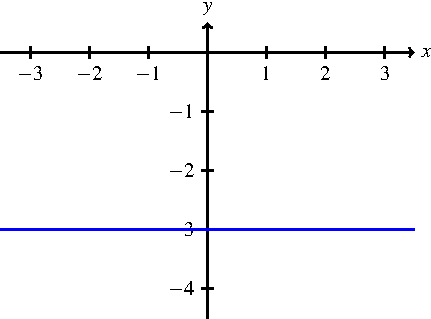
\includegraphics[scale=0.8]{image/06/a-0-b-minus-3.pdf}
}
\caption{%%
  Plots of the constant functions (a)~$f(x) = 2$ and
  (b)~$f(x) = -3$.
}
\label{fig:constant_functions}
\end{figure}

\begin{exercise}
Describe the function $f(x) = -1/2$ and draw its graph.
\end{exercise}

\ifbool{showSolution}{
\begin{solution}
The expression $f(x) = -1/2$ is a constant function.  Its graph is a
horizontal line through the point $-1/2$ on the $y$-axis and this line
is parallel to the $x$-axis.
\Figure{fig:constant_function_minus_half} shows a graph of the
function $f(x)$.
%%
\begin{figure}[!htbp]
\centering
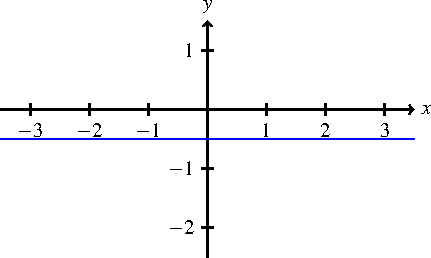
\includegraphics[scale=1]{image/06/a-0-b-minus-half.pdf}
\caption{%%
  A graph of the constant function $f(x) = -1/2$.
}
\label{fig:constant_function_minus_half}
\end{figure}
\end{solution}
}{}

\begin{exercise}
\label{ex:constant_function_zero}
Describe the graph of the expression $f(x) = 0$.
\end{exercise}

\ifbool{showSolution}{
\begin{solution}
The expression $f(x) = 0$ is a constant function whose graph is a
horizontal line through the point $0$ on the $y$-axis.  In other
words, the function $f(x) = 0$ describes the $x$-axis.
\end{solution}
}{}

Now consider the case of $b = 0$ in
\Equation{eqn:linear_function_general} so that you have
$f(x) = ax$.  If you also have $a = 0$, then $f(x)$ is reduced to the
function in \Exercise{ex:constant_function_zero}.  Otherwise assume
that $a \neq 0$.  What does the graph of $f(x) = ax$ look like?

Let's use the strategy from \Section{sec:general_form} to graph
$f(x) = ax$.  Set $f(x) = 0$ and solving the equation $0 = ax$ for $x$
results in $x = 0$.  The $x$-intercept has coordinates
$A = \tuple{0}{0}$.  Next, set $x = 0$ and solving the equation
$y = a \times 0$ for $y$ shows that $y = 0$.  The $y$-intercept is
$B = \tuple{0}{0}$.  Both of $A$ and $B$ are the same point and that
point is the origin.  You need another way to determine a second and
different point of the function $f(x) = ax$.

Instead of setting $x = 0$, you can try setting $x = 1$.  Simplify the
equation $y = a \times 1$ and you obtain $y = a$.  Hence the
second~(and different) point is $\tuple{1}{a}$.  In other words, if
$a \neq 0$ then the graph of $f(x) = ax$ is a straight line that
passes through the origin.  \Figure{fig:function_ax_positive_rational}
shows some graphs of $f(x) = ax$, where $a$ is a positive real number
that is at most $1$, i.e.~$0 < a \leq 1$.
\Figure{fig:function_ax_positive_at_least_one} shows some graphs of
$f(x) = ax$ for the case where $a \geq 1$.  Notice that in both of
these figures, the graphs of $f(x) = ax$ pass through the point
$\tuple{0}{0}$.

\begin{figure}[!htbp]
\centering
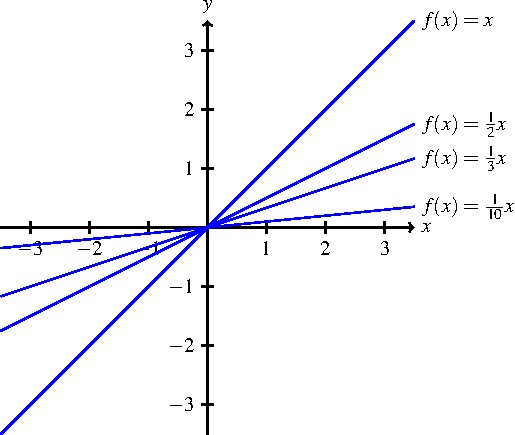
\includegraphics[scale=1]{image/06/ax-small.pdf}
\caption{%%
  Graphs of the function $f(x) = ax$ for various values of $a$, where
  it is assumed that $0 < a \leq 1$.  As the value of $a$ becomes
  smaller and smaller, the graph of $f(x) = ax$ becomes more and more
  like a horizontal line.
}
\label{fig:function_ax_positive_rational}
\end{figure}

\begin{figure}[!htbp]
\centering
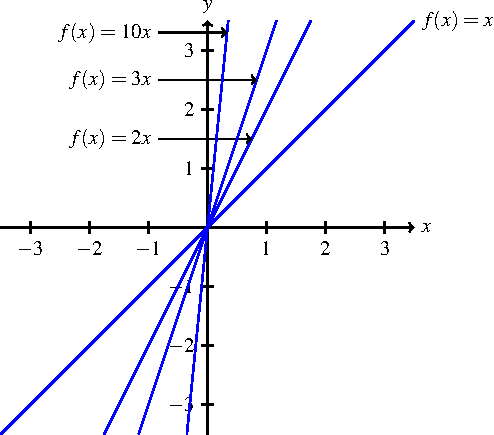
\includegraphics[scale=1]{image/06/ax-large.pdf}
\caption{%%
  Graphs of the function $f(x) = ax$ for various values of $a$, where
  $a \geq 1$.  As the value of $a$ becomes larger and larger, the
  graph of $f(x) = ax$ becomes steeper and steeper like a vertical
  line.
}
\label{fig:function_ax_positive_at_least_one}
\end{figure}

\begin{exercise}
Describe the graphs of the function $f(x) = ax$, where the factor $a$
takes on the values
$a = \quadruple{-\frac{1}{10}}{-\frac{1}{3}}{-\frac{1}{2}}{-1}$.
\end{exercise}

\ifbool{showSolution}{
\begin{solution}
\Figure{fig:graph_ax_a_negative_between_0_minus_1} shows the graphs of
$f(x) = ax$ for the above given values of $a$.  Note that
$-1 \leq a < 0$.  As $a$ becomes larger and larger and approches zero,
the graph of $f(x) = ax$ becomes more and more like a horizontal line.

\begin{figure}[!htbp]
\centering
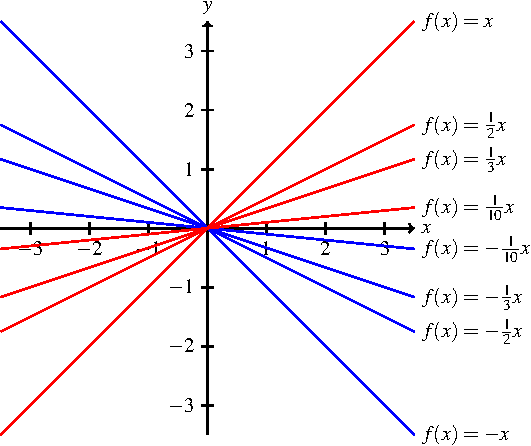
\includegraphics[scale=1]{image/06/ax-small-negative.pdf}
\caption{%%
  The blue lines are graphs of the function $f(x) = ax$, where $a$ has
  the values
  $a = \quadruple{-\frac{1}{10}}{-\frac{1}{3}}{-\frac{1}{2}}{-1}$.
  The red lines are reflections about the $x$-axis of the blue lines.
}
\label{fig:graph_ax_a_negative_between_0_minus_1}
\end{figure}
\end{solution}
}{}

\begin{exercise}
Describe the graphs of the function $f(x) = ax$, where the factor $a$
takes on the values $a = \quadruple{-1}{-2}{-3}{-10}$.
\end{exercise}

\ifbool{showSolution}{
\begin{solution}
\Figure{fig:graph_ax_a_negative_less_than_1} shows the graphs of
$f(x) = ax$ for the above given values of $a$.  Starting from
$a = -1$, as $a$ becomes smaller and smaller, the graph of
$f(x) = ax$ becomes steeper and steeper like a vertical line.

\begin{figure}[!htbp]
\centering
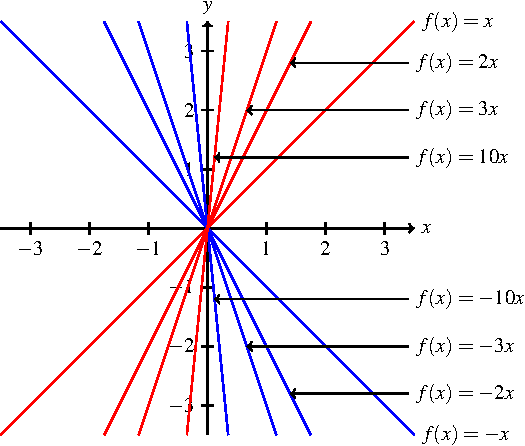
\includegraphics[scale=1]{image/06/ax-large-negative.pdf}
\caption{%%
  The blue lines are graphs of the function $f(x) = ax$, where $a$ has
  the values $a = \quadruple{-1}{-2}{-3}{-10}$.  The red lines are
  reflections about the $x$-axis of the blue lines.
}
\label{fig:graph_ax_a_negative_less_than_1}
\end{figure}
\end{solution}
}{}


%%%%%%%%%%%%%%%%%%%%%%%%%%%%%%%%%%%%%%%%%%%%%%%%%%%%%%%%%%%%%%%%%%%%%%%%%%%

\section{Table of values}

A linear function $f(x) = ax + b$ can also be represented as a table
of values.  The table has two columns.  The left column specifies a
number of values for $x$ and the right column gives the corresponding
values for $f(x)$.  For example, \Table{tab:function_values_a_2_b_1}
shows some values of the function $f(x) = 2x + 1$.  For $x = -3$ you
have the value $f(-3) = 2(-3) + 1 = -6 + 1 = -5$.  For $x = 1$ you
have $f(1) = 2 \times 1 + 1 = 3$.  And so on.

\begin{table}[!htbp]
\centering
\begin{tabular}{rr} \toprule
$x$  & $f(x)$ \\\midrule
$-3$ & $-5$   \\[6pt]
$-2$ & $-3$   \\[6pt]
$-1$ & $-1$   \\[6pt]
$0$  & $1$    \\[6pt]
$1$  & $3$    \\[6pt]
$2$  & $5$    \\[6pt]
$3$  & $7$    \\\bottomrule
\end{tabular}

\caption{%%
  Some specific values of the function $f(x) = 2x + 1$.
}
\label{tab:function_values_a_2_b_1}
\end{table}

\begin{exercise}
Provide a table of values for the function $f(x) = \frac{x}{2} + 2$ at
the values of $x = \quintuple{-2}{-1}{0}{1}{2}$.
\end{exercise}

\ifbool{showSolution}{
\begin{solution}
See \Table{tab:function_values_a_half_b_2}.

\begin{table}[!htbp]
\centering
\begin{tabular}{cc} \toprule
$x$  & $f(x)$  \\\midrule
$-2$ & $1$     \\
$-1$ & $3 / 2$ \\
$0$  & $2$     \\
$1$  & $5 / 2$ \\
$2$  & $3$     \\\bottomrule
\end{tabular}

\caption{%%
  Some values of the function $f(x) = \frac{x}{2} + 2$.
}
\label{tab:function_values_a_half_b_2}
\end{table}
\end{solution}
}{}

\begin{table}[!htbp]
\centering
\begin{tabular}{cc} \toprule
$x$  & $f(x)$   \\\midrule
$0$  & $1 / 2$  \\
$1$  & $7 / 2$  \\
$2$  & $13 / 2$ \\
$3$  & $19 / 2$ \\
$4$  &          \\
$5$  &          \\
$6$  &          \\\bottomrule
\end{tabular}

\caption{%%
  Some values of the function $f(x) = ax + b$.  Fill in the missing
  entries.
}
\label{tab:function_values_a_3_b_half_incomplete}
\end{table}

\begin{exercise}
\Table{tab:function_values_a_3_b_half_incomplete} provides some values
of a linear function $f(x) = ax + b$.  Fill in the missing entries in
the table.
\end{exercise}

\ifbool{showSolution}{
\begin{solution}
You have the difference
$f(1) - f(0) = \frac{7}{2} - \frac{1}{2} = 3$.  Note that you also
have the differences $f(2) - f(1) = 3$ and $f(3) - f(2) = 3$.  Assume
that each time you increase $x$ by one unit, you increase $f(x)$ by
$3$ units to get $f(x + 1)$.  Based upon the latter assumption, you
have $f(4) = f(3) + 3$, $f(5) = f(4) + 3$, and $f(6) = f(5) + 3$.  See
\Table{tab:function_values_a_3_b_half_complete}.

\begin{table}[!htbp]
\centering
\begin{tabular}{cc} \toprule
$x$  & $f(x)$   \\\midrule
$0$  & $1 / 2$  \\
$1$  & $7 / 2$  \\
$2$  & $13 / 2$ \\
$3$  & $19 / 2$ \\
$4$  & $25 / 2$ \\
$5$  & $31 / 2$ \\
$6$  & $37 / 2$ \\\bottomrule
\end{tabular}

\caption{%%
  The same table as \Table{tab:function_values_a_3_b_half_incomplete},
  but with missing values filled in.
}
\label{tab:function_values_a_3_b_half_complete}
\end{table}
\end{solution}
}{}


%%%%%%%%%%%%%%%%%%%%%%%%%%%%%%%%%%%%%%%%%%%%%%%%%%%%%%%%%%%%%%%%%%%%%%%%%%%

\section{Recover a function}

Suppose you are given a table of values and you know that the table
represents a linear function of the form $f(x) = ax + b$.  How would
you determine the values of $a$ and $b$?  You can make two assumptions
about the values in the given table.  Each assumption can be used to
derive a technique that helps you to recover the function $f(x)$.

The first assumption you can make is that the values of $x$ are evenly
spaced and increase by one unit each time.  See the values in
\Table{tab:function_values_a_2_b_minus_1}.  The difference
$f(x + 1) - f(x)$ tells you how many units you add to $f(x)$ when $x$
increases by one unit.  This difference is also the value of $a$ and
for this reason $a$ is also called the \emph{rate of change} of the
function $f(x) = ax + b$.  What remains is to determine the value of
$b$.  From the given table, you pick a value of $x$ and the
corresponding value $f(x)$, substitute those values and the value of
$a$ into the function $f(x) = ax + b$, and solve the equation for
$b$.  In particular, note that if $x = 0$ then
$f(0) = a \times 0 + b = b$ and so the $y$-intercept is
$\tuple{0}{b}$.  In other words, if the given table has the values
$x = 0$ and $f(0)$, you read off the table to obtain $b = f(0)$.
Let's apply the above technique to
\Table{tab:function_values_a_2_b_minus_1}.

\begin{table}[!htbp]
\centering
\begin{tabular}{cc} \toprule
$x$  & $f(x)$ \\\midrule
$0$  & $-1$   \\
$1$  & $1$    \\
$2$  & $3$    \\
$3$  & $5$    \\
$4$  & $7$    \\
$5$  & $9$    \\\bottomrule
\end{tabular}

\caption{%%
  Some values of a linear function $f(x) = ax + b$.
}
\label{tab:function_values_a_2_b_minus_1}
\end{table}

\begin{example}
Suppose the values in \Table{tab:function_values_a_2_b_minus_1} are
generated by a linear function of the form $f(x) = ax + b$.  Determine
the values of $a$ and $b$.
\end{example}

\begin{solution}
First, let's determine the rate of change $a$.  Set $x = 1$ so that
you have the difference
%%
\begin{align*}
f(x + 1) - f(x)
&=
f(1 + 1) - f(1) \\[4pt]
&=
f(2) - f(1) \\[4pt]
&=
3 - 1 \\[4pt]
&=
2
\end{align*}
%%
and so the rate of change is $a = 2$.  Next, you determine the
$y$-intercept $\tuple{0}{b}$.  Note that from
\Table{tab:function_values_a_2_b_minus_1} you have
$f(0) = -1$, which shows that the $y$-intercept has coordinates
$\tuple{0}{-1}$ and so $b = -1$.  You can also derive the value of $b$
by using the value $f(1) = 1$ from
\Table{tab:function_values_a_2_b_minus_1}.  Then you have the equation
$1 = 2 \times 1 + b$, which can be written as $1 = 2 + b$ and solving
for $b$ results in $b = -1$.  Therefore the values in
\Table{tab:function_values_a_2_b_minus_1} can be generated by the
linear function $f(x) = 2x - 1$.
\end{solution}

\begin{table}[!htbp]
\centering
\begin{tabular}{cc} \toprule
$x$  & $f(x)$   \\\midrule
$-1$ & $-1$     \\
$0$  & $1 / 2$  \\
$1$  & $2$      \\
$2$  & $7 / 2$  \\
$3$  & $5$      \\
$4$  & $13 / 2$ \\\bottomrule
\end{tabular}

\caption{%%
  Some values of a linear function $f(x) = ax + b$.
}
\label{tab:function_values_a_3_over_2_b_half}
\end{table}

\begin{exercise}
The values in \Table{tab:function_values_a_3_over_2_b_half} are known
to be values of a linear function of the form $f(x) = ax + b$.
Determine the values of $a$ and $b$ such that $f(x)$ generates the
values in the table.  Derive the value of $b$ in two different ways.
\end{exercise}
%%
\ifbool{showSolution}{
\begin{solution}
Note that in \Table{tab:function_values_a_3_over_2_b_half} the values
of $x$ increase by one unit each time.  First, let's determine the
value of $a$.  Set $x = 0$ and you have the difference
%%
\begin{align*}
f(x + 1) - f(x)
&=
f(0 + 1) - f(0) \\[4pt]
&=
f(1) - f(0) \\[4pt]
&=
2 - \frac{1}{2} \\[4pt]
&=
\frac{4}{2} - \frac{1}{2} \\[4pt]
&=
\frac{3}{2}
\end{align*}
%%
which shows that the rate of change is $a = 3 / 2$.  Next, let's
determine the value of $b$.  From
\Table{tab:function_values_a_3_over_2_b_half} you have the
$y$-intercept $\tuple{0}{\frac{1}{2}}$ and so $b = 1 / 2$.  On the
other hand, you can derive the value of $b$ as follows.  Choose the
value $f(1) = 2$ from \Table{tab:function_values_a_3_over_2_b_half}.
Using the value of $a = 3 / 2$ you have
$2 = \frac{3}{2} \times 1 + b$, which can also be written as
$2 = \frac{3}{2} + b$.  Solve the latter equation for $b$ to get
%%
\begin{align*}
b
&=
2 - \frac{3}{2} \\[4pt]
&=
\frac{4}{2} - \frac{3}{2} \\[4pt]
&=
\frac{1}{2}.
\end{align*}
%%
Therefore the linear function $f(x) = \frac{3}{2}x + \frac{1}{2}$ can
be used to generate the values in
\Table{tab:function_values_a_3_over_2_b_half}.
\end{solution}
}{}

\begin{table}[!htbp]
\centering
\begin{tabular}{cc} \toprule
$x$           & $f(x)$ \\\midrule
$2$           & $-10$  \\[6pt]
$\frac{3}{2}$ & $-8$   \\[6pt]
$\frac{7}{2}$ & $-16$  \\[6pt]
$5$           & $-22$  \\[6pt]
$7$           & $-30$  \\[6pt]
$10$          & $-42$  \\\bottomrule
\end{tabular}

\caption{%%
  Some values of a linear function $f(x) = ax + b$.
}
\label{tab:function_values_a_minus_4_b_minus_2}
\end{table}

The second assumption you can make about a given table of values is
that the values of $x$ are \emph{not} necessarily evenly spaced.  The
values of $x$ in the table can be either evenly spaced or not.
However, the values in the table are assumed to be generated by a
linear function of the form $f(x) = ax + b$ for some constants
$\pair{a}{b} \in \RR$ that are yet to be determined.  See
\Table{tab:function_values_a_minus_4_b_minus_2}.  In this case, you
need a way to calculate the rate of change $a$.  Let $x_1 < x_2$ and
suppose that $f(x_1) = y_1$ and $f(x_2) = y_2$ are two values of the
function $f(x)$ as given in the table.  Since the rate of change is a
constant, it can also be defined as the average value of $f(x)$
between two values of $x$.  In other words, you can write the rate of
change as
%%
\begin{equation}
\label{eqn:linear_function_rate_of_change}
a
=
\frac{
  f(x_2) - f(x_1)
}{
  x_2 - x_1
}
\end{equation}
%%
and this value should be the same no matter what the actual values of
$x_1$, $x_2$, $f(x_1)$, and $f(x_2)$ are.  The value of $b$ can also
be determined as explained above.  An example should help to clarify
the theory.

\begin{example}
Suppose the values in \Table{tab:function_values_a_minus_4_b_minus_2}
are generated by a linear function of the form $f(x) = ax + b$.
Determine the values of $a$ and $b$.
\end{example}

\begin{solution}
First, let's determine the rate of change.  Set $x_1 = 5$ and
$x_2 = 7$ because these values are easy to calculate with.  You should
avoid fractions whenever possible.  Then $f(x_1) = f(5) = -22$ and
$f(x_2) = f(7) = -30$ and substitute these values into
\Equation{eqn:linear_function_rate_of_change} to obtain
%%
\begin{align*}
a
&=
\frac{
  f(7) - f(5)
}{
  7 - 5
} \\[4pt]
&=
\frac{
  -30 - (-22)
}{
  7 - 5
} \\[4pt]
&=
\frac{
  -30 + 22
}{
  7 - 5
} \\[4pt]
&=
\frac{
  -8
}{
  2
} \\[4pt]
&=
-4
\end{align*}
%%
and so the rate of change is $a = -4$.  To calculate the value of $b$,
set $x = 2$ to get $f(2) = -10$ from
\Table{tab:function_values_a_minus_4_b_minus_2}.  Now use the value of
$a$ to write $-10 = -4 \times 2 + b$, which can be simplified to
$-10 = -8 + b$.  Solving the latter equation for $b$ shows that
$b = -10 + 8 = -2$.  Therefore the values in
\Table{tab:function_values_a_minus_4_b_minus_2} can be generated by
the linear function $f(x) = -4x - 2$.
\end{solution}

\begin{table}[!htbp]
\centering
\begin{tabular}{rr} \toprule
$x$            & $f(x)$          \\\midrule
$-\frac{1}{2}$ & $-\frac{25}{6}$ \\[6pt]
$1$            & $-\frac{11}{3}$ \\[6pt]
$\frac{3}{2}$  & $-\frac{7}{2}$  \\[6pt]
$7$            & $-\frac{5}{3}$  \\[6pt]
$12$           & $0$             \\[6pt]
$13$           & $\frac{1}{3}$   \\\bottomrule
\end{tabular}

\caption{%%
  Some values of a linear function $f(x) = ax + b$.
}
\label{tab:function_values_a_third_b_minus_4}
\end{table}

\begin{exercise}
Suppose the values in \Table{tab:function_values_a_third_b_minus_4}
are generated by a linear function of the form $f(x) = ax + b$.
Recover the function $f(x)$ by determining the values of the constants
$a$ and $b$.
\end{exercise}
%%
\ifbool{showSolution}{
\begin{solution}
First, you calculate the rate of change.  Set $x_1 = 12$ and
$x_2 = 13$ and read off \Table{tab:function_values_a_third_b_minus_4}
to get $f(x_1) = f(12) = 0$ and $f(x_2) = f(13) = 1 / 3$.  Use
\Equation{eqn:linear_function_rate_of_change} to write the rate of
change as
%%
\begin{align*}
a
&=
\frac{
  f(13) - f(12)
}{
  13 - 12
} \\[4pt]
&=
\frac{
  \frac{1}{3} - 0
}{
  1
} \\[4pt]
&=
\frac{1}{3}.
\end{align*}
%%
Next, you calculate the value of $b$.  Set $x = 12$ so that
$f(12) = 0$.  Use the known value for the rate of change to obtain the
equation $0 = \frac{1}{3} \times 12 + b$, which simplifies to
$0 = \frac{12}{3} + b$.  Solve the last equation for $b$ and you get
%%
\begin{align*}
b
&=
0 - \frac{12}{3} \\[4pt]
&=
0 - 4 \\[4pt]
&=
-4.
\end{align*}
%%
Therefore the values in \Table{tab:function_values_a_third_b_minus_4}
can be generated by the function $f(x) = \frac{x}{3} - 4$.
\end{solution}
}{}


%%%%%%%%%%%%%%%%%%%%%%%%%%%%%%%%%%%%%%%%%%%%%%%%%%%%%%%%%%%%%%%%%%%%%%%%%%%

\section{Intersection}


%%%%%%%%%%%%%%%%%%%%%%%%%%%%%%%%%%%%%%%%%%%%%%%%%%%%%%%%%%%%%%%%%%%%%%%%%%%

\section*{Problem}

\begin{problem}
\item Let $\quadruple{x_1}{x_2}{y_1}{y_2}$ be real numbers such that
  $x_1 < x_2$.  Consider the two points $A = \tuple{x_1}{y_1}$ and
  $B = \tuple{x_2}{y_2}$ in the Cartesian coordinate system.
  Determine a linear function of the form $f(x) = ax + b$ that passes
  through the points $A$ and $B$.  That is, calculate the values of
  the constants $a$ and $b$.
\ifbool{showSolution}{
\begin{solution}
You have the known values of $f(x_1) = y_1$ and $f(x_2) = y_2$.  Use
\Equation{eqn:linear_function_rate_of_change} to write the rate of
change as
%%
\begin{equation}
\label{eqn:derive_rate_of_change}
\begin{aligned}
a
&=
\frac{
  f(x_2) - f(x_1)
}{
  x_2 - x_1
} \\[4pt]
&=
\frac{
  y_2 - y_1
}{
  x_2 - x_1
}
\end{aligned}
\end{equation}
%%
To calculate the value of $b$, set $x = x_1$ so that $f(x_1) = y_1$.
Use the known value of $a$ to write the equation
$y_1 = ax_1 + b$, which can be solved for $b$ to produce
$b = y_1 - ax_1$ with $a$ as given in
\Equation{eqn:derive_rate_of_change}.
\end{solution}
}{}

\item Going anti-clockwise, there is a span of $\degree{45}$ from the
  positive half of the $x$-axis to the point $A = \tuple{1}{1}$.
  There is a span of $\degree{135}$ from the positive half of the
  $x$-axis to the point $B = \tuple{-1}{1}$, also going
  anti-clockwise.  Let $f(x) = a_1x + b_1$ be a function that passes
  through the point $A$.  Let $g(x) = a_2x + b_2$ be a function that
  passes through the point $B$ such that the straight lines in the
  graphs of $f(x)$ and $g(x)$ are perpendicular to each other.
  Determine two linear functions $f(x)$ and $g(x)$ that satisfy the
  above conditions.
\ifbool{showSolution}{
\begin{solution}
The points $A$ and $B$ are shown in
\Figure{fig:two_points_reflection_each_other_y_axis}, from which you
see that the line segments $OA$ and $OB$ are perpendicular to each
other.  All that you need to do now is to determine a linear function
$f(x)$ that goes through the origin $O$ and the point $A$, and another
linear function $g(x)$ that goes through the origin and the point
$B$.  Note that both linear functions will have the same
$y$-intercept, i.e.~the origin $\tuple{0}{0}$ itself.  Use
\Equation{eqn:derive_rate_of_change} to see that the rate of change of
$f(x)$ is given by
%%
\begin{align*}
a_1
&=
\frac{
  f(1) - f(0)
}{
  1 - 0
} \\[4pt]
&=
\frac{
  1 - 0
}{
  1 - 0
} \\[4pt]
&=
\frac{1}{1} \\[4pt]
&=
1.
\end{align*}
%%
Similarly, the rate of change of $g(x)$ is
%%
\begin{align*}
a_2
&=
\frac{
  g(-1) - g(0)
}{
  -1 - 0
} \\[4pt]
&=
\frac{
  1 - 0
}{
  -1 - 0
} \\[4pt]
&=
\frac{1}{-1} \\[4pt]
&=
-1.
\end{align*}
%%
Therefore the required linear functions are $f(x) = x$ and
$g(x) = -x$.

\begin{figure}[!htbp]
\centering
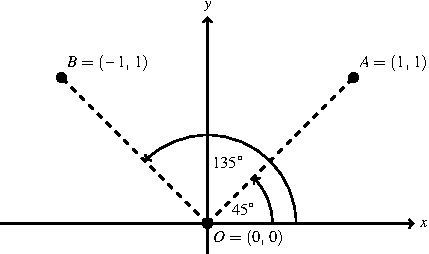
\includegraphics[scale=1.5]{image/06/perpendicular-lines-origin.pdf}
\caption{%%
  Two points that are reflections of each other with respect to the
  $y$-axis.  The angle from the line segment $OA$ to the segment $OB$
  is $\degree{135} - \degree{45} = \degree{90}$, going
  anti-clockwise.  Thus the segments $OA$ and $OB$ are perpendicular
  to each other.
}
\label{fig:two_points_reflection_each_other_y_axis}
\end{figure}
\end{solution}
}{}

\begin{table}[!htbp]
\centering
\begin{tabular}{cc} \toprule
Celsius $C$  & Fahrenheit $F(C)$ \\\midrule
$10$ & $50$ \\
$15$ & $59$ \\
$20$ & $68$ \\
$25$ & $77$ \\
$30$ & $86$ \\
$35$ & $95$ \\\bottomrule
\end{tabular}

\caption{%%
  Temperature conversion from degree Celsius to degree Fahrenheit.
}
\label{tab:temperature_Celsius_to_Fahrenheit}
\end{table}

\item \Table{tab:temperature_Celsius_to_Fahrenheit} shows how to
  convert between degrees Celsius and Fahrenheit.  Assume that the
  conversion from Celsius to Fahrenheit is given by a linear function
  of the form $F(C) = aC + b$, where $C$ represents the degree in
  Celsius and $F(C)$ represents the degree in Fahrenheit.  Determine
  the values of the constants $a$ and $b$.
\ifbool{showSolution}{
\begin{solution}
First, determine the rate of change.
\Table{tab:temperature_Celsius_to_Fahrenheit} shows that $F(10) = 50$
and $F(15) = 59$.  Use \Equation{eqn:linear_function_rate_of_change}
to write the rate of change as
%%
\begin{align*}
a
&=
\frac{
  F(15) - F(10)
}{
  15 - 10
} \\[4pt]
&=
\frac{
  59 - 50
}{
  15 - 10
} \\[4pt]
&=
\frac{9}{5}.
\end{align*}
%%
Next, determine the value of $b$.  Set $C = 10$ to get $F(10) = 50$.
Use the value of $a$ to write $50 = \frac{9}{5} \times 10 + b$, which
you can simplify to $50 = 9 \times 2 + b$ or $50 = 18 + b$.  Solving
the last equation for $b$ shows that $b = 50 - 18 = 32$.  Therefore
the conversion from degree Celsius to degree Fahrenheit is given by
the linear function $F(C) = \frac{9}{5} C + 32$.
\end{solution}
}{}

\begin{table}[!htbp]
\centering
\begin{tabular}{rc} \toprule
$x$  & $f(x)$ \\\midrule
$0$  & $1$    \\[6pt]
$1$  & $3$    \\[6pt]
$4$  & $5$    \\[6pt]
$9$  & $7$    \\[6pt]
$16$ & $9$    \\\bottomrule
\end{tabular}

\caption{%%
  Some values of an unknown function $f(x)$.  Is the function $f(x)$
  linear?
}
\label{tab:non_linear_function}
\end{table}

\item \Table{tab:non_linear_function} shows some values of a function
  $f(x)$.  You do not know a formula for $f(x)$.  However, you want to
  know whether the function $f(x)$ is linear.  Explain two different
  ways to help you decide whether $f(x)$ is linear.
\ifbool{showSolution}{
\begin{solution}
Suppose the values in \Table{tab:non_linear_function} are generated by
a function $f(x)$.  One way to decide whether the function $f(x)$ is
linear is to sketch the given points on one set of coordinate axes.
See \Figure{fig:plot_non_linear_function}.  If $f(x)$ is linear, you
would expect its graph to be one straight line going through the five
points given in \Table{tab:non_linear_function}.  However,
\Figure{fig:plot_non_linear_function} shows that the given points can
be joined up by multiple straight lines.  So from
\Figure{fig:plot_non_linear_function} you may conclude that the values
in \Table{tab:non_linear_function} are generated by a function that is
not linear.

To be absolutely sure that the function $f(x)$ is not linear, you can
use \Equation{eqn:linear_function_rate_of_change} to calculate the
rate of change for two different pairs of points.  If $f(x)$ is
linear, you would expect $f(x)$ to have exactly one rate of change.
Let's calculate the rate of change by using the points $\tuple{0}{1}$
and $\tuple{1}{3}$.  These two points result in the rate of change
%%
\begin{align*}
\frac{
  f(1) - f(0)
}{
  1 - 0
}
&=
\frac{
  3 - 1
}{
  1
} \\[4pt]
&=
\frac{
  2
}{
  1
} \\[4pt]
&=
2.
\end{align*}
%%
Let's calculate the rate of change by using the different points
$\tuple{4}{5}$ and $\tuple{9}{7}$.  The latter pair of points results
in the rate of change
%%
\begin{align*}
\frac{
  f(9) - f(4)
}{
  9 - 4
}
&=
\frac{
  7 - 5
}{
  5
} \\[4pt]
&=
\frac{
  2
}{
  5
}
\end{align*}
%%
which is different from the rate of $2$ that you calculated above.
Therefore the function $f(x)$ that generated the data in
\Table{tab:non_linear_function} is not linear.

\begin{figure}[!htbp]
\centering
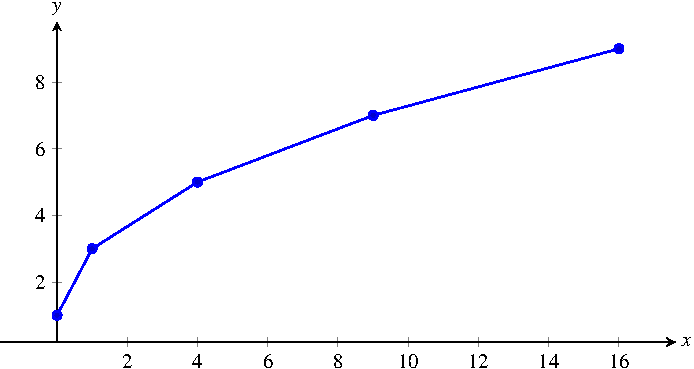
\includegraphics[scale=1]{image/06/nonlinear.pdf}
\caption{%%
  A plot of the data points from \Table{tab:non_linear_function}.
}
\label{fig:plot_non_linear_function}
\end{figure}
\end{solution}
}{}
\end{problem}

\end{document}
